%% 
%% Copyright 2007-2025 Elsevier Ltd
%% 
%% This file is part of the 'Elsarticle Bundle'.
%% ---------------------------------------------
%% 
%% It may be distributed under the conditions of the LaTeX Project Public
%% License, either version 1.3 of this license or (at your option) any
%% later version.  The latest version of this license is in
%%    http://www.latex-project.org/lppl.txt
%% and version 1.3 or later is part of all distributions of LaTeX
%% version 1999/12/01 or later.
%% 
%% The list of all files belonging to the 'Elsarticle Bundle' is
%% given in the file `manifest.txt'.
%% 
%% Template article for Elsevier's document class `elsarticle'
%% with numbered style bibliographic references
%% SP 2008/03/01
%% $Id: elsarticle-template-num.tex 272 2025-01-09 17:36:26Z rishi $
%%
%\documentclass[preprint,12pt]{elsarticle}
\documentclass[final,1p,times,review]{elsarticle}

%% Use the option review to obtain double line spacing
%% \documentclass[authoryear,preprint,review,12pt]{elsarticle}

%% Use the options 1p,twocolumn; 3p; 3p,twocolumn; 5p; or 5p,twocolumn
%% for a journal layout:
%% \documentclass[final,1p,times]{elsarticle}
%% \documentclass[final,1p,times,twocolumn]{elsarticle}
%% \documentclass[final,3p,times]{elsarticle}
%% \documentclass[final,3p,times,twocolumn]{elsarticle}
%% \documentclass[final,5p,times]{elsarticle}
%% \documentclass[final,5p,times,twocolumn]{elsarticle}

%% For including figures, graphicx.sty has been loaded in
%% elsarticle.cls. If you prefer to use the old commands
%% please give \usepackage{epsfig}

%% The amssymb package provides various useful mathematical symbols
\usepackage{amssymb}
%% The amsmath package provides various useful equation environments.
\usepackage{amsmath}
%% The amsthm package provides extended theorem environments
%% \usepackage{amsthm}
\usepackage{algorithm}
\usepackage[caption=false]{subfig}
\usepackage{subfloat}
\usepackage{xcolor}
\usepackage{hyperref}
\usepackage{rotating}
\usepackage{booktabs}   
\usepackage{colortbl}  
\usepackage{physics}  
\usepackage{appendix}

%% The lineno packages adds line numbers. Start line numbering with
%% \begin{linenumbers}, end it with \end{linenumbers}. Or switch it on
%% for the whole article with \linenumbers.
%% \usepackage{lineno}

\usepackage{lineno}
% \linenumbers

\journal{Journal of Computational Physics}

\begin{document}

\begin{frontmatter}

	%% Title, authors and addresses

	%% use the tnoteref command within \title for footnotes;
	%% use the tnotetext command for theassociated footnote;
	%% use the fnref command within \author or \affiliation for footnotes;
	%% use the fntext command for theassociated footnote;
	%% use the corref command within \author for corresponding author footnotes;
	%% use the cortext command for theassociated footnote;
	%% use the ead command for the email address,
	%% and the form \ead[url] for the home page:
	%% \title{Title\tnoteref{label1}}
	%% \tnotetext[label1]{}
	%% \author{Name\corref{cor1}\fnref{label2}}
	%% \ead{email address}
	%% \ead[url]{home page}
	%% \fntext[label2]{}
	%% \cortext[cor1]{}
	%% \affiliation{organization={},
	%%             addressline={},
	%%             city={},
	%%             postcode={},
	%%             state={},
	%%             country={}}
	%% \fntext[label3]{}

	\title{A unified second-order immersed-boundary and ghost-fluid method on a single Cartesian mesh for the Vlasov–Poisson system with complex boundaries}

	%% use optional labels to link authors explicitly to addresses:
	%% \author[label1,label2]{}
	%% \affiliation[label1]{organization={},
	%%             addressline={},
	%%             city={},
	%%             postcode={},
	%%             state={},
	%%             country={}}
	%%
	%% \affiliation[label2]{organization={},
	%%             addressline={},
	%%             city={},
	%%             postcode={},
	%%             state={},
	%%             country={}}

	\author[UVA]{Hunt Feng\fnref{hf_label}} %% Author name
	\fntext[hf_label]{Visiting Researcher, University of Virginia}
	% Hunt, if you need any other affiliations, feel free to add them below and then add back the label in front of your name

	\author[UVA]{Haibo Dong\fnref{hd_label}} %% Author name
	\fntext[hd_label]{Professor, University of Virginia}
	%% Author affiliation


	\author[UVA]{Chen Cui\corref{cor1}\fnref{cc_label}} %% Author name
	\ead{cuichen@virginia.edu}
	\fntext[cc_label]{Assistant Professor, University of Virginia}
	\cortext[cor1]{Corresponding author}
	%% Author affiliation


	%% Author affiliation
	\affiliation[UVA]{organization={Department of Mechanical and Aerospace Engineering, University of Virginia},%Department and Organization
		addressline={122 Engineer's Way},
		city={Charlottesville},
		postcode={22904},
		state={VA},
		country={USA}}


	%% Abstract
	\begin{abstract}
		Plasma-material interactions are critical to applications from electric propulsion and spacecraft charging to fusion divertor erosion and semiconductor fabrication. Predictive modeling requires high-fidelity, fully kinetic simulations that resolve the velocity distribution function (VDF) near complex boundaries. Particle-in-Cell (PIC) methods are widely used but suffer from noise and poor sampling of high-energy tails, where key plasma–surface processes occur. Grid-based Vlasov method avoids these issues by directly solving the VDF, but faces challenges imposing sharp, curved geometries on Cartesian meshes without costly local refinement.

		We present a unified, second-order immersed-boundary framework for the 2D2V Vlasov-Poisson system on a single Cartesian grid. A ghost-fluid method enforces dielectric jump conditions between plasma and solid in the Poisson solver, while a sharp-interface ghost-cell scheme applies complex geometry conditions for the Vlasov equation without staircasing errors or dual meshes. Coupled with a Positive Flux Conserving semi-Lagrangian scheme, our method ensures charge conservation, VDF positivity, and relaxed CFL limits.

		This approach enables accurate, noise-free kinetic simulations in complex geometries, resolving high-energy tails and near-wall structures. Results on classical plasma-dielectric cases demonstrate robust handling of curved boundaries, opening a practical path for Vlasov modeling in real-world applications.
	\end{abstract}

	%%Graphical abstract
	%\begin{graphicalabstract}
	%%\includegraphics{grabs}
	%\end{graphicalabstract}

	%%Research highlights
	%\begin{highlights}
	%\item Research highlight 1
	%\item Research highlight 2
	%\end{highlights}

	%% Keywords
	\begin{keyword}
		%% keywords here, in the form: keyword \sep keyword

		%% PACS codes here, in the form: \PACS code \sep code

		%% MSC codes here, in the form: \MSC code \sep code
		%% or \MSC[2008] code \sep code (2000 is the default)
		Semi-Lagrangian scheme \sep Immersed boundary method \sep Vlasov-Poisson system \sep Ghost fluid method \sep Plasma-material interaction
	\end{keyword}

\end{frontmatter}

%% Add \usepackage{lineno} before \begin{document} and uncomment 
%% following line to enable line numbers
%% \linenumbers

%% main text
%%
\section{Introduction}
Grid-based kinetic plasma simulations based on the Vlasov equation evolve the distribution function directly in phase space rather than sampling it with numerical particles. In contrast to particle-in-cell (PIC) methods, the continuum approach is free of sampling noise and therefore gives direct access to fine distribution-function structure, weak phase-space features, and wall fluxes. For that reason, continuum kinetic methods are especially attractive in bounded plasma problems where sheath structure, non-Maxwellian features, and plasma-material interaction must be resolved with high fidelity. 

One of the main obstacles for applying the Vlasov method in the real engineering is geometric complexity. In a Vlasov solver, the physical-space mesh is coupled to a discretization in velocity space, and every additional cost in configuration space is effectively replicated across the velocity grid. As a result, design choices that are common in CFD, such as body-fitted meshes, heavy local refinement near curved walls, or distinct meshes for transport and field equations, can become much more expensive and much harder to manage in the grid-based kinetic computations. Recent high-order GPU work on Vlasov-Poisson solvers again highlights that the very large number of phase-space unknowns is a central practical limitation of the grid-based kinetic methods.

One possible approach for resolving this issue is to use body-fitted or unstructured meshes directly in phase space. This direction was explored early, for example, by Besse and Sonnendrücker, who developed semi-Lagrangian Vlasov schemes on unstructured phase-space meshes. However, the literature also makes clear why this route is difficult to scale in arbitrary geometry. Filbet and Yang explicitly argued that, because of the high-dimensional nature of kinetic equations, unstructured-mesh treatments are often unattractive and that Cartesian-grid techniques are preferable when possible. For Vlasov solvers, this argument is particularly compelling because many high-order Eulerian and semi-Lagrangian algorithms derive much of their efficiency from structured-grid operations.

On the other hand, a uniform mesh with arbitrary boundary condition can be a promising approach. More recently, Liu et al. developed an immersed finite element and conservative semi-Lagrangian framework for plasma-material interaction on structured interface-independent meshes, combining a first order half-way ghost-cell treatment for Vlasov transport with an immersed field solve. These works clearly demonstrate progress, but they also show that the design space remains open, particularly for time-dependent, same-mesh, sharp-interface Vlasov–Poisson formulations with explicit near-boundary accuracy analysis.

A closely related body of work exists in deterministic rarefied-gas simulation, where discrete-velocity and BGK/Boltzmann solvers face a very similar tension between velocity-space cost and geometric fidelity. There, Cartesian embedded-boundary ideas have proved especially attractive. Mieussens’ survey emphasized immersed Cartesian techniques as a promising direction for deterministic solvers. Filbet and Yang developed an inverse Lax-Wendroff boundary treatment for Boltzmann-type models in arbitrary geometry on Cartesian meshes. Dechriste and Mieussens later showed that conservative Cartesian cut-cell methods can combine geometric flexibility, exact conservation, and a relatively simple implementation for rarefied flows around moving obstacles. This rarefied-gas literature strongly suggests that a Cartesian sharp-interface treatment is a natural strategy for grid-based Vlasov solvers as well.

The contribution of the present work is therefore not simply to introduce complex geometry into Vlasov simulation, since that topic has already seen meaningful progress, but to provide a unified same-mesh formulation in which both the Vlasov and Poisson equations are treated with second-order sharp-interface accuracy near the boundary. This is particularly useful when the interior Vlasov solver is of higher order: a second-order near-boundary closure is accurate enough to remain consistent with the interior discretization on practical meshes, while avoiding the very dense local refinement that would otherwise be required around curved objects. 

The remainder of the paper is organized as follows. Section 2 introduces the mathematical model and boundary conditions. Section 3 presents the unified same-mesh numerical method. Section 4 discusses the consistency and accuracy analysis near the immersed boundary. Section 5 contains numerical verification and validation. Section 6 presents representative application cases. Section 7 concludes the paper.

\section{Governing Equations and Problem Setting}
\subsection{Vlasov-Poisson System}
This part introduces the Vlasov-Poisson system

\subsection{Nondimensionalization and geometry representation}

\subsection{Boundary conditions}
Mathematically define the boundary condition for Poisson and Vlasov

\section{Unified IBM and GFM Numerical Method}

\subsection{Governing equations}

Assuming a collisionless plasma, the evolution of the distribution function for particle species $s$ is governed by the Vlasov equation:
\begin{equation}
	\label{eq:vlasov}
	\partial_t f_s + \mathbf{v} \cdot \nabla_{\mathbf{x}} f_s + \left(\frac{q_s}{m_s}\mathbf{E}\right)\cdot \nabla_{\mathbf{v}} f_s = 0.
\end{equation}

The \textit{Vlasolver} solves the Vlasov--Poisson system by coupling a kinetic solver for Eq.~\eqref{eq:vlasov} with a field solver for the Poisson equation.

\subsection{Unified coupling framework}

We introduce a cell-centered Cartesian mesh (Fig.~\ref{fig:unified_mesh}), which is shared by both the Vlasov and Poisson solvers. As illustrated in Fig.~\ref{fig:unified_mesh}, both the distribution function and the electrostatic potential are defined at cell centers, enabling a consistent and efficient data exchange between the two solvers.

\begin{figure}[htbp]
	\centering
	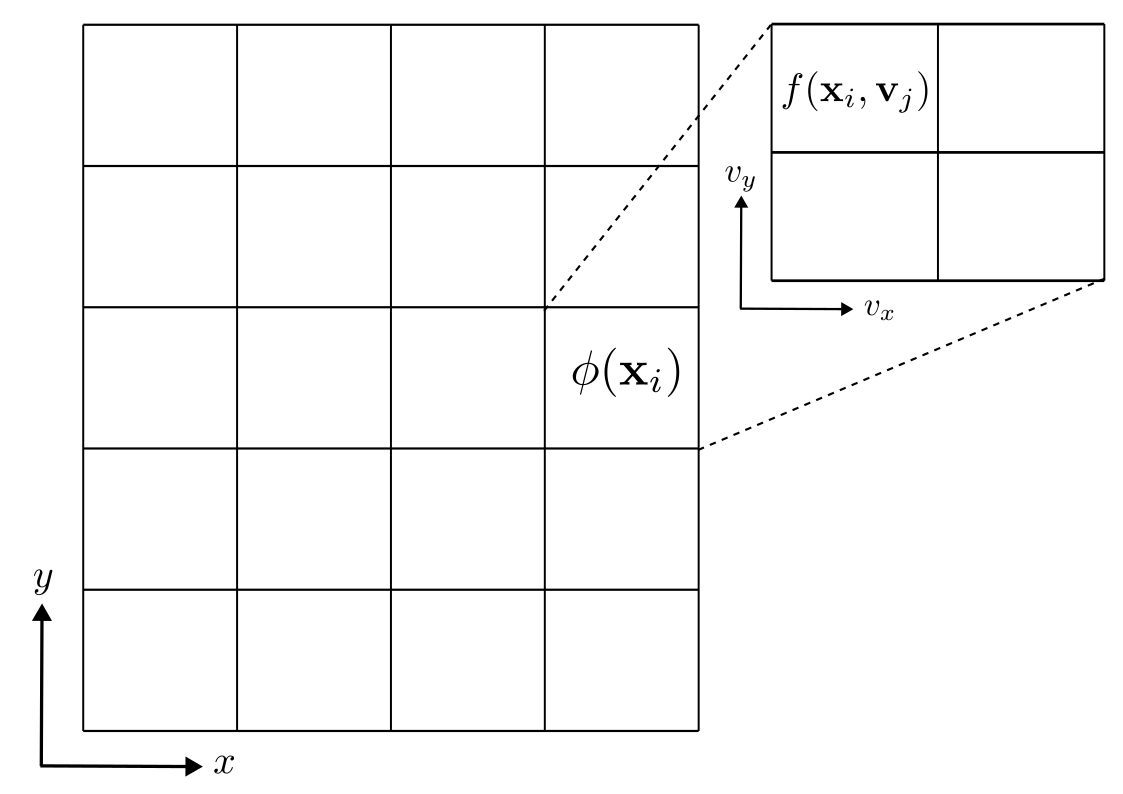
\includegraphics[width=0.6\textwidth]{figures/unified_mesh.png}
	\caption{Schematic of the unified cell-centered mesh used for both the Vlasov and Poisson solvers.}
	\label{fig:unified_mesh}
\end{figure}

The Vlasov equation is discretized using a semi-Lagrangian scheme based on the positive flux-conservative (PFC) formulation. The primary unknown is the cell-averaged distribution function:
\begin{equation}
	f_{ij}^n = \frac{1}{\Delta x \Delta v}
	\int_{x_{i-1/2}}^{x_{i+1/2}}
	\int_{v_{j-1/2}}^{v_{j+1/2}}
	f(\mathbf{x}, \mathbf{v}, t^n)\, \mathrm{d}x\, \mathrm{d}v.
\end{equation}

The scheme advances these cell averages directly, ensuring conservation and positivity without explicitly evaluating the integrals during time evolution.

The electrostatic potential is computed by solving the Poisson equation using a finite-difference method on the same mesh. The charge density is obtained from velocity moments of the distribution function:
\begin{equation}
	\rho(\mathbf{x}) = \sum_s q_s \int f_s(\mathbf{x}, \mathbf{v})\, \mathrm{d}\mathbf{v}.
\end{equation}

The overall coupling procedure is illustrated in Fig.~\ref{fig:coupling_scheme}. At each time step, the Vlasov solver updates the distribution function using the electric field, while the Poisson solver computes the electric field from the charge density. This establishes a self-consistent evolution of particles and fields.

\begin{figure}[htbp]
	\centering
	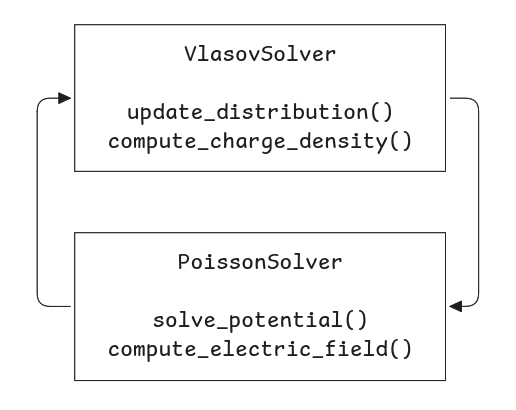
\includegraphics[width=0.75\textwidth]{figures/coupling_scheme.png}
	\caption{Flowchart of the coupling between the Vlasov and Poisson solvers in the Vlasolver framework.}
	\label{fig:coupling_scheme}
\end{figure}

\subsection{Vlasov solver}
A well known second order time integration technique called Strang splitting is applied to the Vlasov equation. This technique splits the Vlasov equation into two advection equations, one in the position space and the other in the velocity space.

\begin{align}
	\label{eq:spatial_advection}
	\partial_t f + \mathbf{v}_s\cdot\grad_{\mathbf{x}} f_s = 0 \\
	\label{eq:velocity_advection}
	\partial_t f + (q_s\mathbf{E}/m_s)\cdot\grad_{\mathbf{v}} f_s = 0
\end{align}

Then update the two advection equations in the following orders:

\begin{equation}
	\label{eq:strang-splitting}
	\begin{aligned}
		f_s^{*}(\mathbf{x}, \mathbf{v})   & = f_s^n(\mathbf{x} - \mathbf{v}_s\Delta t/2, \mathbf{v}),           \\
		f_s^{**}(\mathbf{x}, \mathbf{v})  & = f_s^{*}(\mathbf{x}, , \mathbf{v}- (q_s\mathbf{E}/m_s)\Delta t/2), \\
		f_s^{n+1}(\mathbf{x}, \mathbf{v}) & = f_s^{**}(\mathbf{x} - \mathbf{v}_s\Delta t/2, \mathbf{v}).
	\end{aligned}
\end{equation}

In each step, the advection update is performed using a 3rd-order PFC scheme.

\subsection{PFC scheme for advection update}
Notice that the spatial and velocity advection equations both take the form
\begin{equation}
	\partial_t f + \partial_x(vf) = 0,
	\label{eq:advection_simplified}
\end{equation}
where $v$ denotes as velocity $\mathbf{v}$ in Eq.~(\ref{eq:spatial_advection}) or acceleration $q\mathbf{E}/m$ in Eq.~(\ref{eq:velocity_advection}). A PFC scheme is implemented to solve such advection equation.

On a uniform cell-centered mesh defined on computational domain $[x_{\text{min}}, x_{\text{max}}]$. The cell centers are defined as $x_i = x_{\text{min}} + (i+1/2)\Delta x$, where $\Delta x$ is the cell size. We use $f_i^n=\int_{x_{i-1/2}}^{x_{i+1/2}} f(x,t^n)\dd x/\Delta x$ to denote the average distribution function at the $i$-th cell center and time step $n$.

The PFC scheme updates the distribution function at the next time step, $f_i^{n+1}$, by tracing the characteristic line back to the previous time step, $t^n$,

\begin{equation}
	\int_{x_{i-1/2}}^{x_{i+1/2}} f(x, t^{n+1}) \dd x = \int_{x_{i-1/2} - v\Delta t}^{x_{i+1/2} - v\Delta t} f(x, t^n) \dd x.
	\label{eq:trace_characteristic}
\end{equation}

Meaning that the cell-averaged distribution function at the next time step, $f_i^{n+1}$, can be evaluated by

\begin{equation}
	f_i^{n+1} = f_i^n + F_{i-1/2} - F_{i+1/2}.
	\label{eq:distribution_update}
\end{equation}
where $F_{i-1/2} = \int_{x_{i-1/2} - v\Delta t}^{x_{i-1/2}} f(x, t^n) \dd x/\Delta x$ and $F_{i+1/2}=\int_{x_{i+1/2} - v\Delta t}^{x_{i+1/2}} f(x, t^n) \dd x/\Delta x$ are the fluxes through the cell left and right interfaces.

The flux can approximated by a 3rd-order scheme,
\begin{equation}
	F_{i+1/2} = \begin{cases}
		\abs{\varphi}\left( f_{j}^n + \frac{1}{6}(2 - \abs{\varphi})(1-\abs{\varphi})(f_{j+1}^n - f_{j}^n) + \frac{1}{6}(1 - \abs{\varphi})(1+\abs{\varphi})(f_{j}^n - f_{j-1}^n)\right), & \varphi > 0, \\
		\abs{\varphi}\left( f_{j}^n + \frac{1}{6}(2 - \abs{\varphi})(1-\abs{\varphi})(f_{j}^n - f_{j-1}^n) + \frac{1}{6}(1 - \abs{\varphi})(1+\abs{\varphi})(f_{j+1}^n - f_{j}^n)\right), & \varphi < 0.
	\end{cases}
	\label{eq:flux_3rd_order}
\end{equation}
where $\varphi = v\Delta t/\Delta x$ is related to CFL number, and $j = i - \lfloor\varphi\rfloor$.

To preserve positivity of the distribution function, a flux limiter described in \cite{liu2021conservative} is applied to the flux,
\begin{equation}
	\hat{F}_{i+1/2} = L_{i+1/2} \left( F_{i+1/2} - f_{i+1/2} \right) + f_{i+1/2}.
	\label{eq:modified_flux}
\end{equation}

The $L_{i+1/2} = \min(L_i^r, L_{i+1}^l)$, where
\begin{equation}
	L_i^l =
	\begin{cases}
		\min\left(1, \delta_i^k/d_{i-1/2} \right), & d_{i-1/2} < 0 \text{ and } d_{i+1/2} < 0,     \\
		\delta_i^k/(d_{i-1/2} - d_{i+1/2}),        & d_{i-1/2} d_{i+1/2} < 0 \text{ and } p_i < 0, \\
		1,                                         & \text{else},
	\end{cases}
	\label{eq:flux_limiter_left}
\end{equation}

\begin{equation}
	L_i^r =
	\begin{cases}
		\min\left(1, -\delta_i^k/d_{i+1/2} \right), & d_{i-1/2} \ge 0 \text{ and } d_{i+1/2} > 0,   \\
		\delta_i^k/(d_{i-1/2} - d_{i+1/2}),         & d_{i-1/2} d_{i+1/2} < 0 \text{ and } p_i < 0, \\
		1,                                          & \text{else},
	\end{cases}
	\label{eq:flux_limiter_right}
\end{equation}

where $f_{i+1/2} = \varphi f_i^n$ is the first order flux, and $\epsilon_{i+1/2}\in[0,1]$ is the positivity-preserving limiter to ensure the positivity of the function $f_{i}^{n+1}$ in Eq.~(\ref{eq:distribution_update}). We denote $d_{i\pm1/2} = F_{i\pm1/2} - f_{i\pm1/2}$ and $p_i = d_{i-1/2} - d_{i+1/2} -\delta_i^n$.

Finally, the new update scheme for the distribution function is
\begin{equation}
	f_i^{n+1} = f_i^n + \hat{F}_{i -1/2} - \hat{F}_{i+1/2}.
	\label{eq:final_update}
\end{equation}

\subsection{Immersed boundary treatment for the Vlasov solver}

The computational domain is partitioned into fluid, solid, and ghost cells. As shown in Fig.~\ref{fig:ibm_2nd_order}, ghost cells are solid cells adjacent to the interface that are used to enforce boundary conditions.

\begin{figure}[htbp]
	\centering
	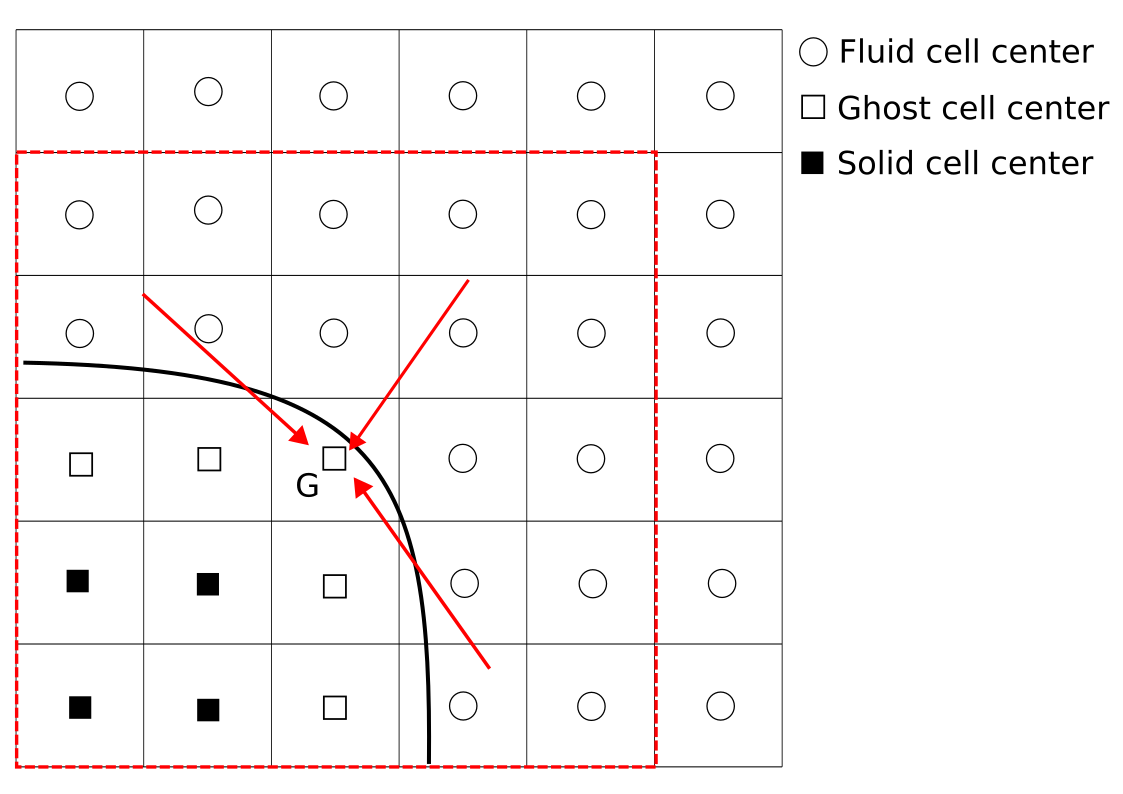
\includegraphics[width=0.6\textwidth]{figures/immersed_boundary_2nd_order.png}
	\caption{Illustration of cell classification and interface representation in the immersed boundary method.}
	\label{fig:ibm_2nd_order}
\end{figure}

The interface is implicitly represented, and its intersection with grid lines defines interface points $\mathbf{x}_I$. At each interface point, the outward normal vector $\mathbf{n}$ is computed to distinguish inflow and outflow directions in velocity space.

The boundary condition is imposed directly on the distribution function at interface points. The treatment depends on the sign of $\mathbf{v}\cdot \mathbf{n}$:

\begin{itemize}
	\item \textbf{Outflow ($\mathbf{v}\cdot \mathbf{n} < 0$):}
	      The distribution function is extrapolated from interior fluid values.

	\item \textbf{Inflow ($\mathbf{v}\cdot \mathbf{n} > 0$):}
	      A fully absorbing boundary condition is imposed, i.e., $f(\mathbf{x}_I, \mathbf{v}) = 0$.
\end{itemize}

This directional treatment ensures consistency with the kinetic transport mechanism and avoids unphysical reflections at the boundary.

Once the interface values are determined, ghost-cell values are reconstructed to complete the numerical stencil. As illustrated in Fig.~\ref{fig:ibm_2nd_order}, the ghost value is obtained by extrapolation using the nearby fluid cells.

Given a range for extrapolation (Fig.~\ref{fig:ibm_2nd_order}), the coefficients, $c_0$, $c_1$ and $c_2$ are determined by the distribution function at near-by fluid cells, which are selected based on the shape of the immersed object. Then solving a least-square problem we can obtain the coefficients,

\begin{equation}
	\min_{c_0,c_1,c_2} \sum_{k=1}^{N_F} (c_0 + c_1x_k + c_2y_k - f_k)^2
	\label{eq:least_square_matrix}
\end{equation}
where $N_F$ is the number of near-by fluid cells in the extrapolation range, and $f_k$ is the distribution function at the $k$-th near-by fluid cell.

\begin{equation}
	f(\mathbf{x}_G, \mathbf{v}, t) = \begin{cases}
		0                              & , \mathbf{v}\cdot\mathbf{n} > 0, \\
		\max(c_0 + c_1x_G + c_2y_G, 0) & , \mathbf{v}\cdot\mathbf{n} < 0.
	\end{cases}
	\label{eq:extrapolation}
\end{equation}

\subsection{Second-order ghost-fluid treatment for the Poisson equation}

We consider the elliptic interface problem on a 2D domain $\Omega \subset \mathbb{R}^2$:
\begin{align}
	\nabla \cdot (\epsilon \nabla \phi) & = f \quad \text{in } \Omega \setminus \Gamma, \\
	[\phi]                              & = a \quad \text{on } \Gamma,                  \\
	[\epsilon \partial_n \phi]          & = b \quad \text{on } \Gamma,
\end{align}
where $\Gamma$ is an interface separating $\Omega$ into $\Omega^+$ and $\Omega^-$, and $[q] = q^+ - q^-$ denotes the jump. The unit normal vector is computed by
\begin{align}
	\mathbf{n} = \frac{\nabla \eta}{|\nabla \eta|}.
\end{align}

Throughout the discussion, we assume $\epsilon$ is piecewise constant and $a,b$ are given functions defined on the interface. The normal vector components $n_x$ and $n_y$ are approximated by fourth-order central differences of the level set function $\eta$.

\subsubsection{Finite Difference Discretization}

Away from the interface, the equation is discretized using standard second-order central differences:
\begin{equation}
	\begin{aligned}
		 & \frac{1}{\Delta x}
		\left[
			\epsilon_{i+\frac{1}{2},j} \frac{\phi_{i+1,j} - \phi_{i,j}}{\Delta x}
			-
			\epsilon_{i-\frac{1}{2},j} \frac{\phi_{i,j} - \phi_{i-1,j}}{\Delta x}
		\right]               \\
		+
		 & \frac{1}{\Delta y}
		\left[
			\epsilon_{i,j+\frac{1}{2}} \frac{\phi_{i,j+1} - \phi_{i,j}}{\Delta y}
			-
			\epsilon_{i,j-\frac{1}{2}} \frac{\phi_{i,j} - \phi_{i,j-1}}{\Delta y}
			\right] = f_{i,j}.
	\end{aligned}
\end{equation}

\subsubsection{Interface Treatment via Boundary Condition Capturing}

For each grid point $(i,j)$ near the interface, define four directional points:
\begin{align}
	x_R & = (x_i + \theta_R \Delta x, y_j), \quad
	x_L = (x_i - \theta_L \Delta x, y_j),         \\
	x_T & = (x_i, y_j + \theta_T \Delta y), \quad
	x_B = (x_i, y_j - \theta_B \Delta y),
\end{align}
where $\theta \in (0,1]$ gives the fractional distance to the interface, computed from the level set function using quadratic interpolation. For example, if $(x_i, y_j)\in\Omega^-$, then

\begin{equation}
	\theta_R = \begin{cases}
		1                                                                                   & , \eta_{i+1,j}\eta_{i,j} > 0 \\
		\frac{-D_x^0\eta + \sqrt{(D_x^0\eta)^2 - 4(D_{xx}^0\eta)\eta_{i,j}}}{2D_{xx}^0\eta} & , \eta_{i+1,j}\eta_{i,j} < 0
	\end{cases},
	\label{eq:theta_computation}
\end{equation}
where $D_{xx}^0\eta = (\eta_{i-1,j}-2\eta_{i,j}+\eta_{i+1,j})/2$ and $D_x^0\eta = (\eta_{i+1,j}-\eta_{i-1,j})/2$. For $\mathbf{x}_L, \mathbf{x}_T$ and $\mathbf{x}_B$, and the case where $(x_i, y_j)\in\Omega^+$ are computed similarly.


\subsubsection{Second-Order Interface Reconstruction}

At an interface point (e.g. $\mathbf{x}_R$), denote the one-sided values by $\phi^-_R$ and $\phi^+_R$. These are determined by enforcing:
\begin{align}
	[\phi](\mathbf{x}_I)            & = a_I, \\
	[\epsilon \phi_n](\mathbf{x}_I) & = b_I,
\end{align}
where $a_I$ is approximated by cubic interpolation of $b_{i-1}, b_{i}, b_{i+1}, b_{i+2}$ and so is $b_I$.

\subsubsection{Modified Discrete Operator}

The final discrete equation at $(i,j)$ becomes:
\begin{equation}
	\begin{aligned}
		 & \left[
			\epsilon_{i+\theta_R/2,j} \frac{\phi_R - \phi_{i,j}}{\theta_R \Delta x}
			-
			\epsilon_{i-\theta_L/2,j} \frac{\phi_{i,j} - \phi_L}{\theta_L \Delta x}
			\right]
		\left/ \left(\frac{\theta_R+\theta_L}{2} \Delta x\right) \right. \\
		+
		 & \left[
			\epsilon_{i,j+\theta_T/2} \frac{\phi_T - \phi_{i,j}}{\theta_T \Delta y}
			-
			\epsilon_{i,j-\theta_B/2} \frac{\phi_{i,j} - \phi_B}{\theta_B \Delta y}
			\right]
		\left/ \left(\frac{\theta_T+\theta_B}{2} \Delta y\right) \right.
		= f_{i,j},
	\end{aligned}
	\label{eq:modified_poisson}
\end{equation}
where $\phi_R, \phi_L, \phi_T, \phi_B$ are either:
\begin{itemize}
	\item standard cell values (no interface crossing), or
	\item interface values expressed in terms of neighboring cell values.
\end{itemize}

\subsubsection{Solving for Interface Ghost Fluid Values}

In 2D, the normal derivative jump condition $[\epsilon \phi_n]$ are expressed in terms of Cartesian derivatives as $[\epsilon \phi_x]$ and $[\epsilon \phi_y]$. We have two different approaches to compute $[\epsilon \phi_x]$ and $[\epsilon \phi_y]$: One from the normal/tangential jumps and the other from a second-order polynomial reconstruction of $\phi$ in $\Omega^-$. By equating these two different discretizations, we can solve for the unknown interface values $\phi_R^-, \phi_L^-, \phi_T^-, \phi_B^-$.

In 2D, jumps in Cartesian derivatives are related to normal/tangential jumps:
\begin{equation}
	\begin{aligned}
		[\epsilon \phi_x] & = [\epsilon \phi_n] n_x - [\epsilon \phi_\tau] n_y                               \\
		                  & = [\epsilon \phi_n] n_x - [\epsilon]\phi_\tau^- n_y - \epsilon^+ [\phi]_\tau n_y \\
		                  & = [\epsilon \phi_n] n_x - [\epsilon]\phi_\tau^+ n_y - \epsilon^- [\phi]_\tau n_y
		\label{eq:poisson_derivative_jump_x}
	\end{aligned}
\end{equation}
and
\begin{equation}
	\begin{aligned}
		[\epsilon \phi_y] & = [\epsilon \phi_n] n_y + [\epsilon \phi_\tau] n_x                                \\
		                  & = [\epsilon \phi_n] n_y + [\epsilon]\phi_\tau^- n_x + \epsilon^+ [\phi]_\tau n_x  \\
		                  & = [\epsilon \phi_n] n_y + [\epsilon]\phi_\tau^+ n_x + \epsilon^- [\phi]_\tau n_x,
		\label{eq:poisson_derivative_jump_y}
	\end{aligned}
\end{equation}
where the following identity was used:
\begin{equation}
	[pq] = [p]q^- + p^+[q].
\end{equation}
Since $[\phi] = a$, so $[\phi]_\tau \approx a_\tau$. The discretization of $a_\tau$ is obtained by applying fourth-order central differences to the $a$,
\begin{equation}
	(a_\tau)_{i,j} = -(D_xa)(n_y)_{i,j} + (D_ya)(n_x)_{i,j},
\end{equation}
where $D_xa=(-a_{i+2,j}+8a_{i+1,j}-8a_{i-1,j}+a_{i-2,j})/12\Delta x$, $D_ya=(-a_{i,j+2}+8a_{i,j+1}-8a_{i,j-1}+a_{i,j-2})/12\Delta y$.

Let $\mathbf{x}_{\text{ext}} = (x_{\text{ext}},y_{\text{ext}})$ be any of the four points $(x_{i-1}, y_{j-1}), (x_{i+1}, y_{j-1}), (x_{i-1}, y_{j+1}),(x_{i+1}, y_{j+1})$ belonging to $\Omega^-$. $\phi_{\text{ext}}$ refers to the value of $\phi$ at $\mathbf{x}_{\text{ext}}$. Then, consider a quadratic polynomial $P(x,y) = Ax^2 + Bxy + Cy^2 + Dx + Ey + F$ that satisfies that interpolates:
\begin{equation}
	\begin{aligned}
		P(\mathbf{x}_T)            & = \phi_T^-,          \\
		P(\mathbf{x}_B)            & = \phi_B^-,          \\
		P(\mathbf{x}_L)            & = \phi_L^-,          \\
		P(\mathbf{x}_R)            & = \phi_R^-,          \\
		P(x_i,y_j)                 & = \phi_{i,j},        \\
		P(\mathbf{x}_{\text{ext}}) & = \phi_{\text{ext}}.
	\end{aligned}
\end{equation}
We can always express the coefficients of polynomial $P$ in terms of $\phi_T^-, \phi_B^-, \phi_L^-, \phi_R^-, \phi_{i,j}, \phi_{\text{ext}}$ by solving the above linear system.

Finally, Eq.~(\ref{eq:poisson_derivative_jump_x}) can be approximated by
\begin{equation}
	[\epsilon \phi_x] \approx [\epsilon \phi_n] n_x - [\epsilon]\left(\grad{P}\cdot\tau\right)n_y - \epsilon^+ a_\tau n_y.
	\label{eq:poisson_derivative_jump_x_geometry}
\end{equation}
In the computation, $b, n_x, n_y, a_\tau$ are approximated by cubic interpolation of quantities defined at mesh cells.

Suppose the interface lies at $\mathbf{x}_{i,j} + \mathbf{x}_R$, then substitute $\phi_L = \phi_{i-1,j}, \phi_T=\phi_{i,j+1}, \phi_B=\phi_{i,j-1}$ into Eq.~(\ref{eq:poisson_derivative_jump_x_geometry}), we can express $[\epsilon \phi_x]$ in terms of $\phi_R^-$ and neighboring cell values. This gives us one approximation of $[\epsilon \phi_x]$ at $\mathbf{x}_R$.

On the other hand, the jump $[\epsilon \phi_x](\mathbf{x}_R)$ by definition is
\begin{equation}
	[\epsilon \phi_x]_R = \eval{\epsilon^+\phi_x^+ - \epsilon^-\phi_x^-}_{\mathbf{x}_R}.
\end{equation}
Therefore, $[\epsilon \phi_x]$ can be approximated by approximating $\phi^+$ and $\phi^-$ using second order finite differences.

By equating the two different approximations of $[\epsilon \phi_x]$,
\begin{equation}
	\eval{\epsilon^+\phi_x^+ - \epsilon^-\phi_x^-}_{\mathbf{x}_R} \approx \eval{[\epsilon \phi_n] n_x - [\epsilon]\left(\grad{P}\cdot\tau\right)n_y - \epsilon^+ a_\tau n_y}_{\mathbf{x}_R},
	\label{eq:equate_derivative_jump}
\end{equation}
we can solve for the unknown interface value $\phi_R^-$. Similarly, by equating the two different approximations of $[\epsilon \phi_x](\mathbf{x}_L)$, we can solve for $\phi_L^-$. Same procedure applies to $\phi_T^-$ and $\phi_B^-$.

Once we obtain the expression of $\phi_R^-, \phi_L^-, \phi_T^-, \phi_B^-$ in terms of neighboring cell values, we can substitute them into the modified discrete operator in Eq.~(\ref{eq:modified_poisson}) to obtain a linear system for $\mathbf{\phi} = [...,\phi_{i,j},...]^T$ at all cells. This linear system is solved by a preconditioned GEMRES solver.

\section{Numerical analysis of the scheme}
\subsection{Accuracy of the Vlasov IBM}
Both mathematically show the accuracy of the constructed scheme 

\subsection{Accuracy of the Poisson GFM}
Mathematically show the accuracy of the constructed scheme
\section{Numerical verification and validation}
\subsection{Manufactured solution for the immersed Vlasov equation}

We first verify the advection part of the solver in the absence of external forces.
The governing equation reduces to a pure 2D2V advection problem:
\begin{equation}
\frac{\partial f}{\partial t}
+ v_x \frac{\partial f}{\partial x}
+ v_y \frac{\partial f}{\partial y}
= 0,
\end{equation}
where \(f = f(x,y,v_x,v_y,t)\) is the distribution function.

The physical domain is \([0,1] \times [0,0.5]\) and the velocity domain is \([-0.05, 0.95] \times [-0.5, 0.5]\).  
Periodic boundary conditions are imposed in all phase‑space directions.  
An absorbing cylinder is defined by the level‑set function
\(\eta(x,y) = (x-0.375)^2 + y^2 - 0.125^2\); on this immersed boundary the distribution function is set to zero.

The initial condition is a Gaussian pulse in \(x\) and a Dirac delta in velocity,
\begin{equation}
f(x,y,v_x,v_y,0) =
\frac{1}{\Delta v_x \Delta v_y}\,
\exp\!\left(-\left(\frac{x - x_0}{0.05}\right)^{\!2}\right)
\delta(v_x-C,\, v_y),
\end{equation}
where \(\delta\) denotes the two‑dimensional Dirac delta, \(C\) is a constant drift velocity, and \(\Delta v_x,\Delta v_y\) are the velocity grid spacings (the factor \(1/(\Delta v_x\Delta v_y)\) approximates the delta in the discrete setting).  
Thus, the particles move with constant velocity in the \(x\) direction, and the Poisson equation is disabled.

This configuration benchmarks the ability of the scheme to capture advection, interaction with an immersed boundary, and particle loss due to absorption as the pulse propagates across the domain and encounters the cylinder.  
The convergence study (Fig.~\ref{fig:advection_convergence}) shows that the solver recovers third‑order accuracy in free space and second‑order accuracy near the immersed boundary.

\begin{figure}[htbp!]
	\centering
	\subfloat[Number density]{
		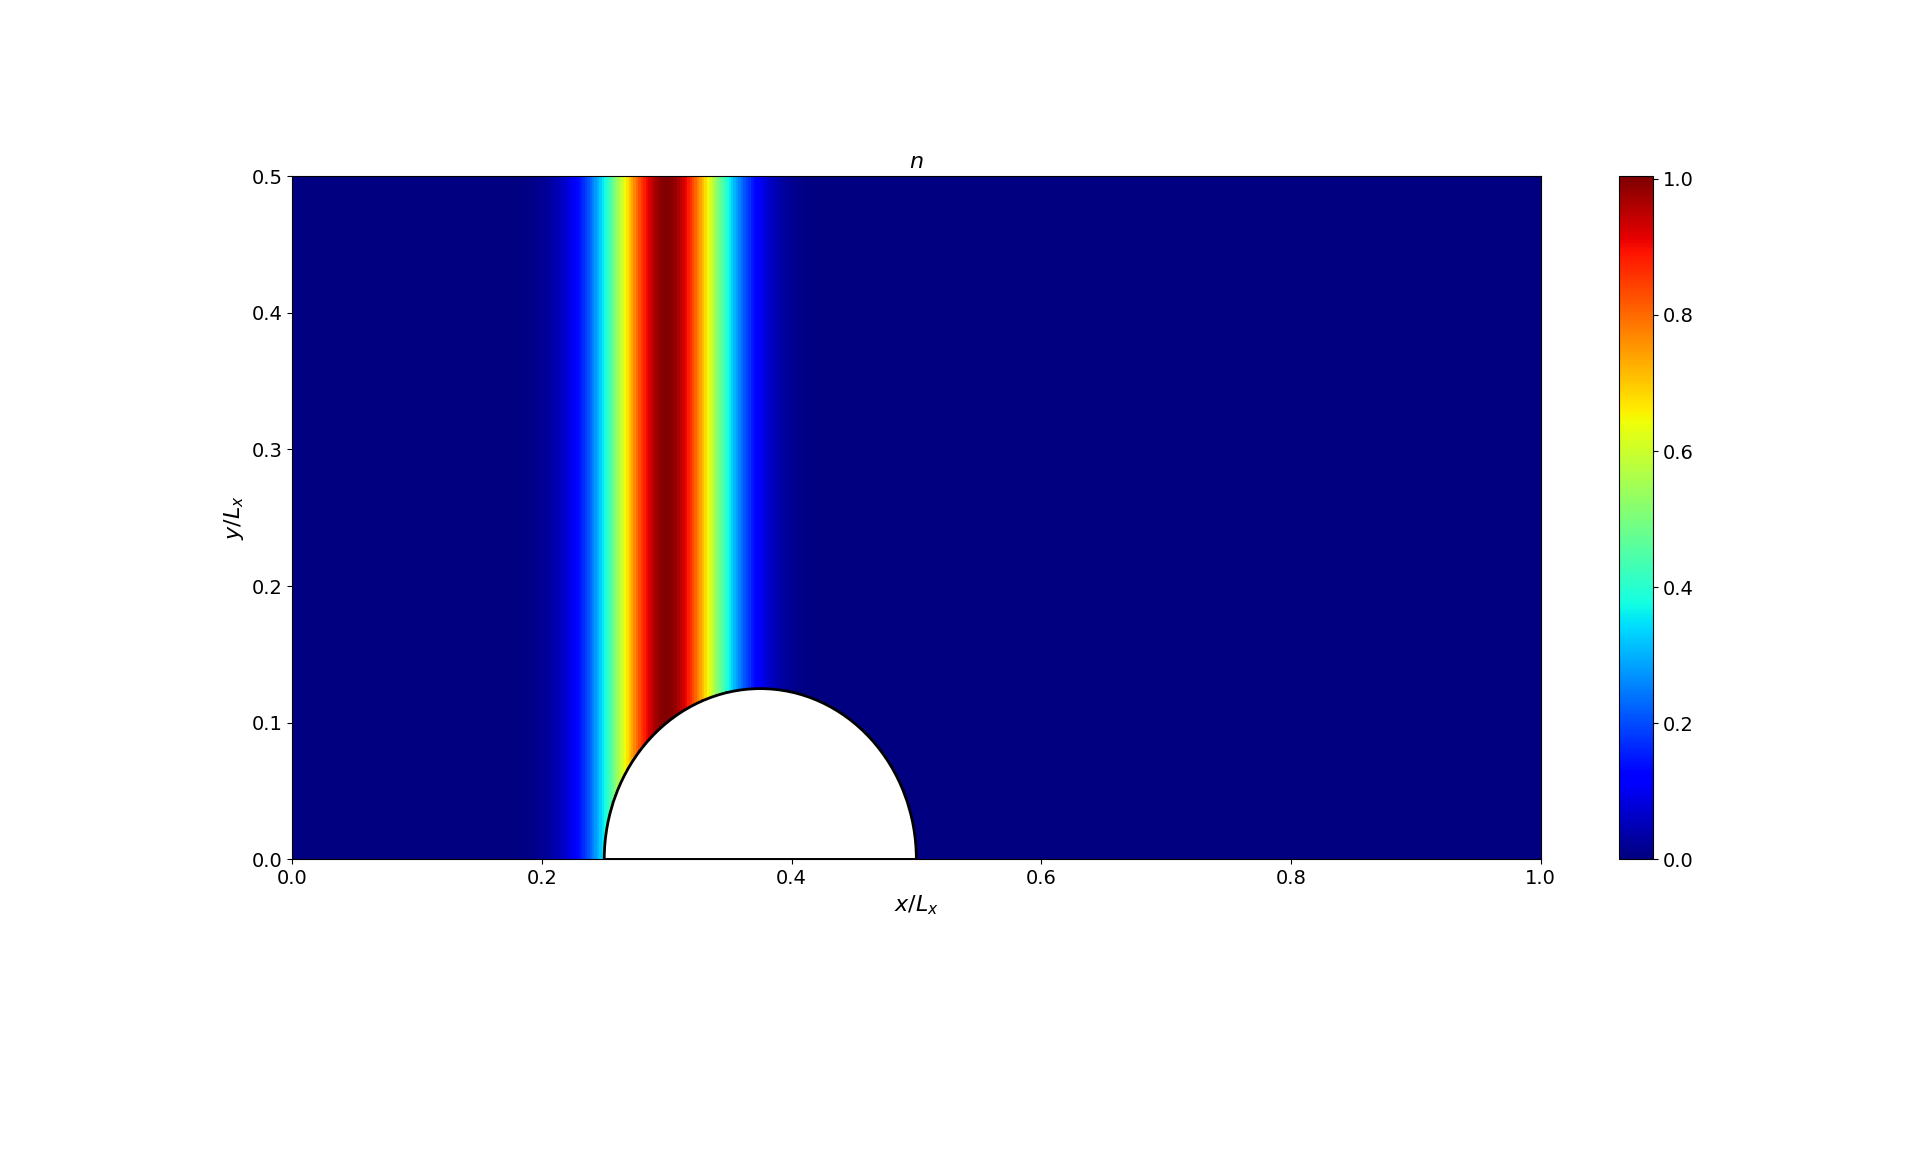
\includegraphics[width=0.5\textwidth]{figures/advection_number_density.png}
	}
	\subfloat[Number density profiles]{
		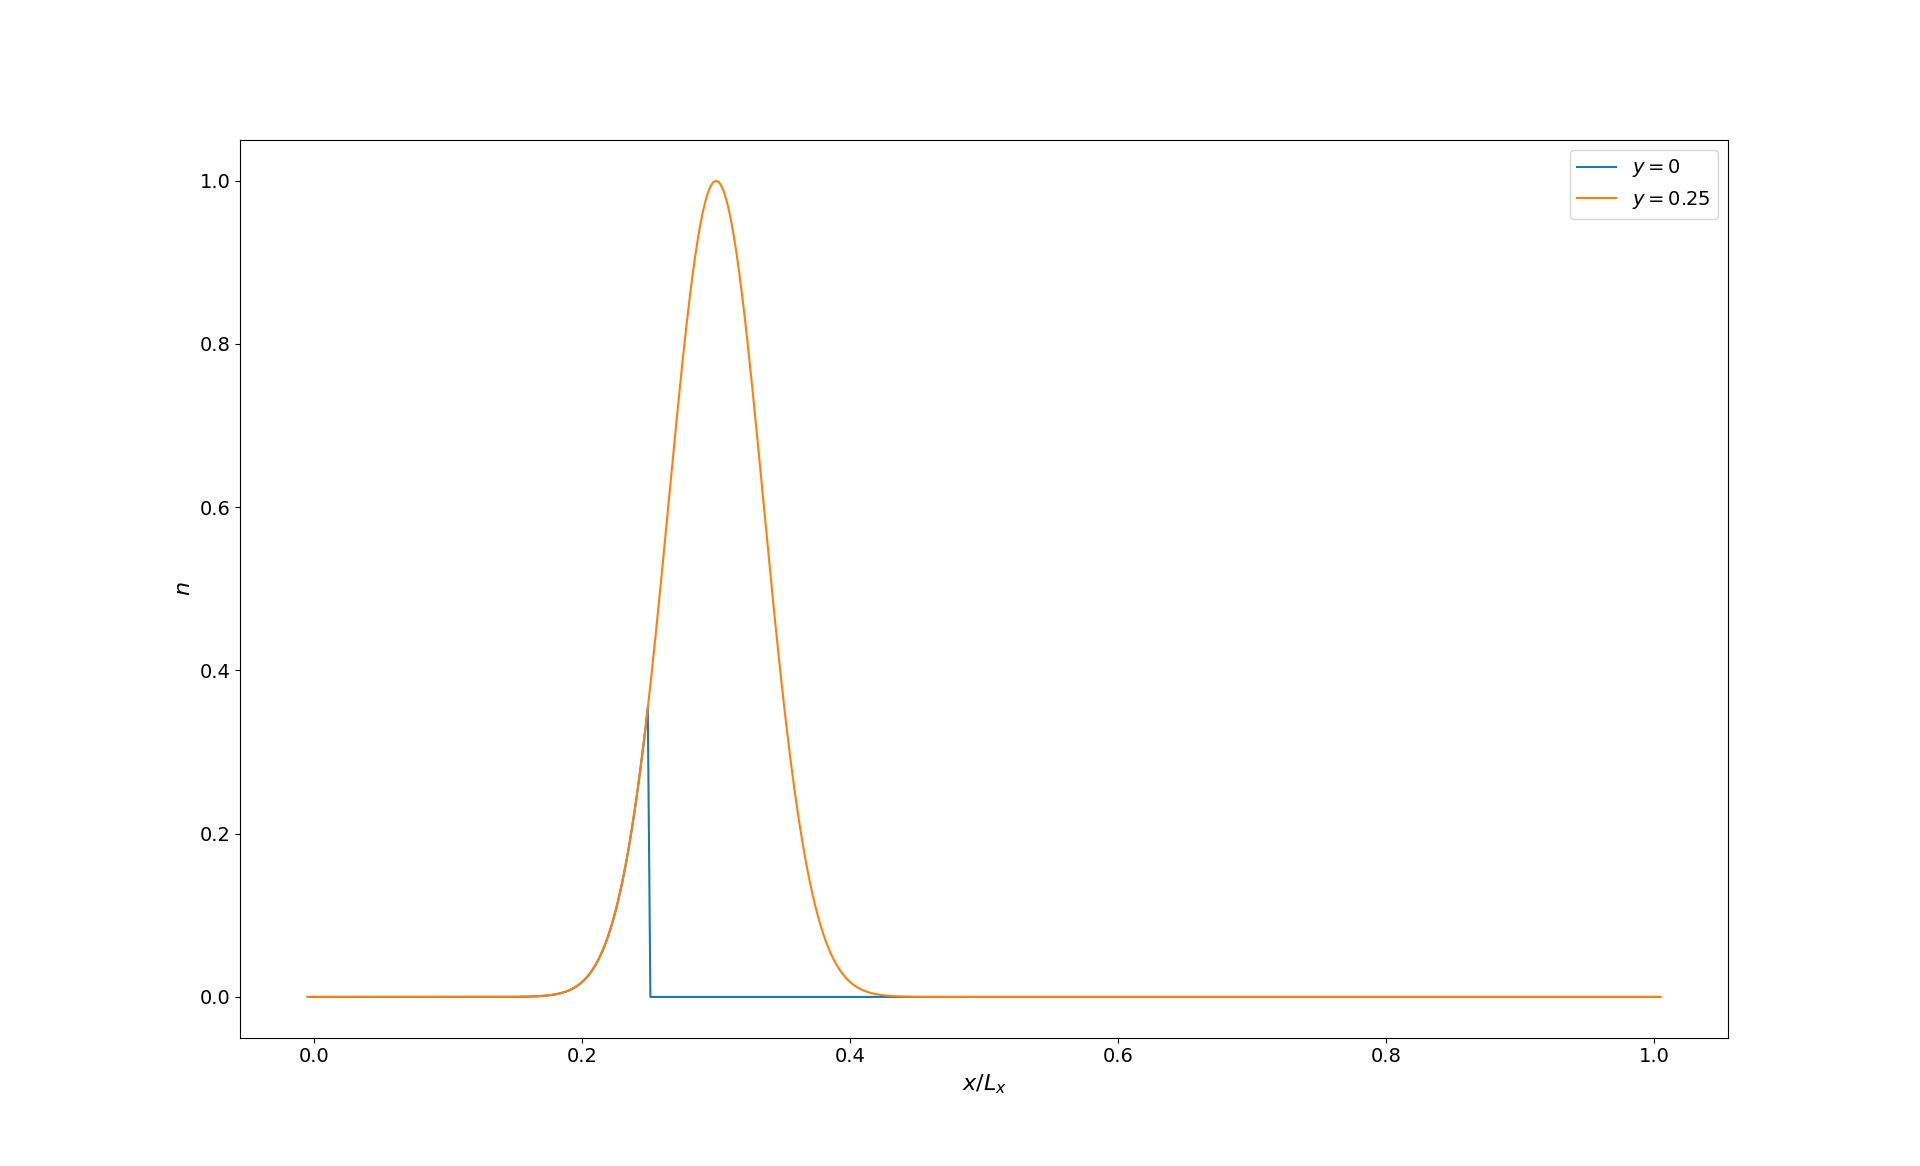
\includegraphics[width=0.5\textwidth]{figures/advection_number_density_profiles.png}
	}
	\label{fig:advection}
\end{figure}

\begin{figure}[htbp!]
	\centering
	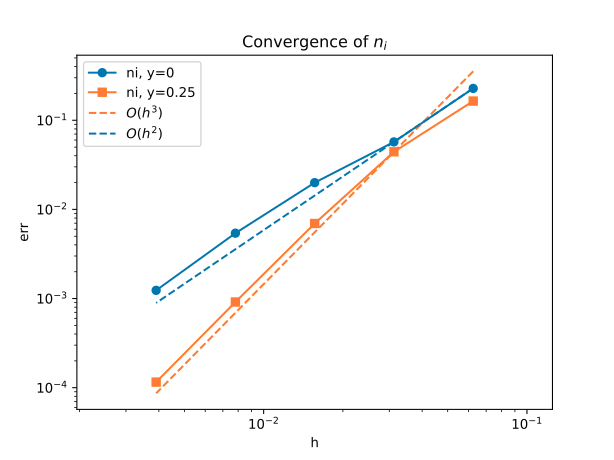
\includegraphics[width=\textwidth]{figures/convergence_advection.png}
	\caption{Convergence study: second‑order accuracy is achieved near the immersed boundary.}
	\label{fig:advection_convergence}
\end{figure}


\subsection{Manufactured solution for the Poisson equation}

Having verified the advection solver, we now turn off the advection and examine the accuracy and convergence order of the Poisson solver in isolation.

The computational domain is \(\Omega = [0,1] \times [0,1]\) with homogeneous Dirichlet conditions on the outer boundary.  
An immersed circular interface \(\Gamma\) is introduced via the level‑set function
\(\eta(x,y) = (x - 0.5)^2 + (y - 0.5)^2 - 0.25^2\).  
The permittivity \(\epsilon\) jumps across \(\Gamma\):
\begin{equation}
\epsilon(x,y) =
\begin{cases}
2, & (x,y) \in \Omega^{-}, \\
1, & (x,y) \in \Omega^{+},
\end{cases}
\end{equation}
where \(\Omega^{-}\) is the interior of the circle and \(\Omega^{+}\) the exterior.  
A charge density is defined only inside the immersed region:
\begin{equation}
\rho(x,y) =
\begin{cases}
-8\,(x^2 + y^2 - 1)\,\exp\big(-(x^2 + y^2)\big), & (x,y) \in \Omega^{-}, \\
0, & (x,y) \in \Omega^{+}.
\end{cases}
\end{equation}

To test the accuracy of the Poisson solver with jump conditions, we prescribe the potential jump and the surface charge density on \(\Gamma\):
\begin{align}
[\phi]_\Gamma &= -\exp\big(-(x^2 + y^2)\big), \\
\left[ \epsilon \frac{\partial \phi}{\partial n} \right]_\Gamma
&=
8\,(2x^2 + 2y^2 - x - y)\,
\exp\big(-(x^2 + y^2)\big).
\end{align}

The convergence study (Fig.~\ref{fig:poisson_convergence}) demonstrates that the solver attains second‑order accuracy even in the presence of these jumps.

\begin{figure}[htbp!]
	\centering
	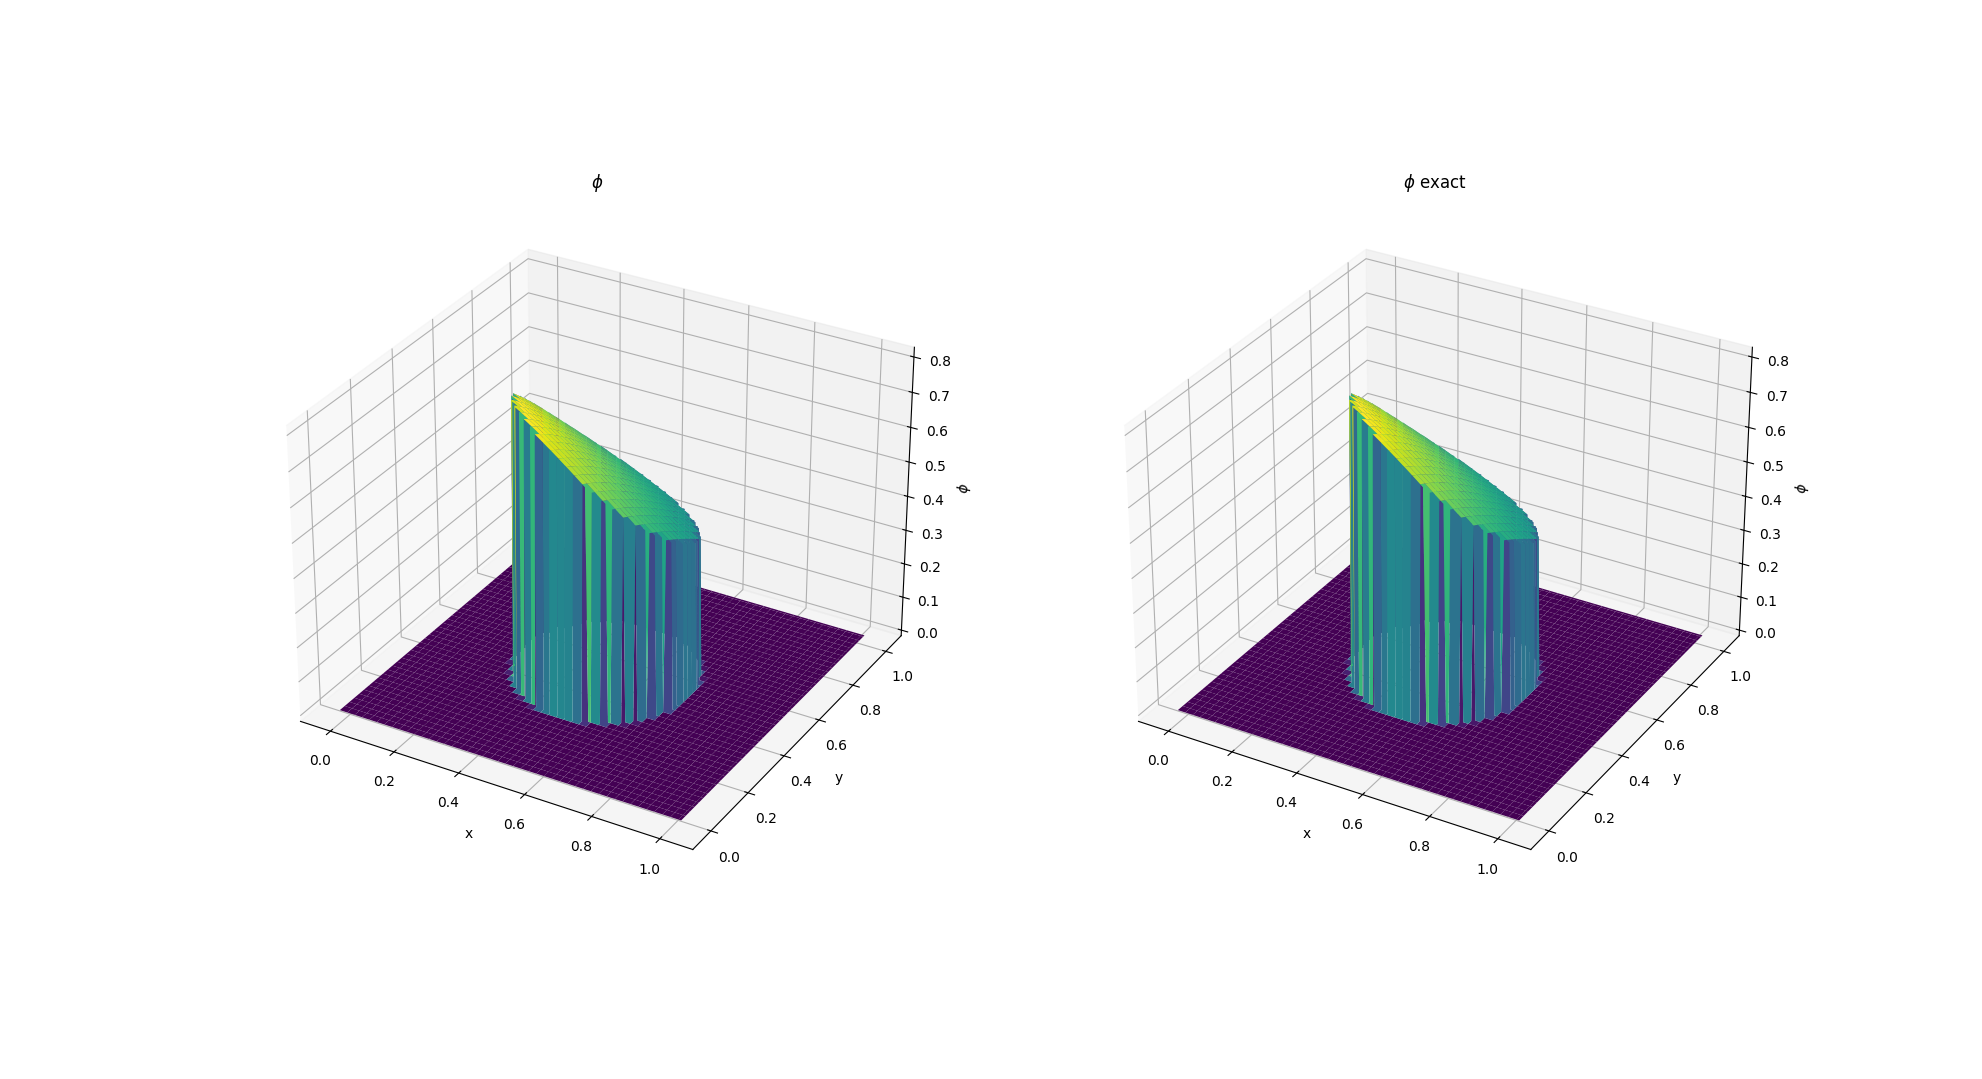
\includegraphics[width=\textwidth]{figures/poisson_solution.png}
	\caption{Numerical solution of the Poisson equation for the manufactured problem.}
	\label{fig:poisson_solution}
\end{figure}

\begin{figure}[htbp!]
	\centering
	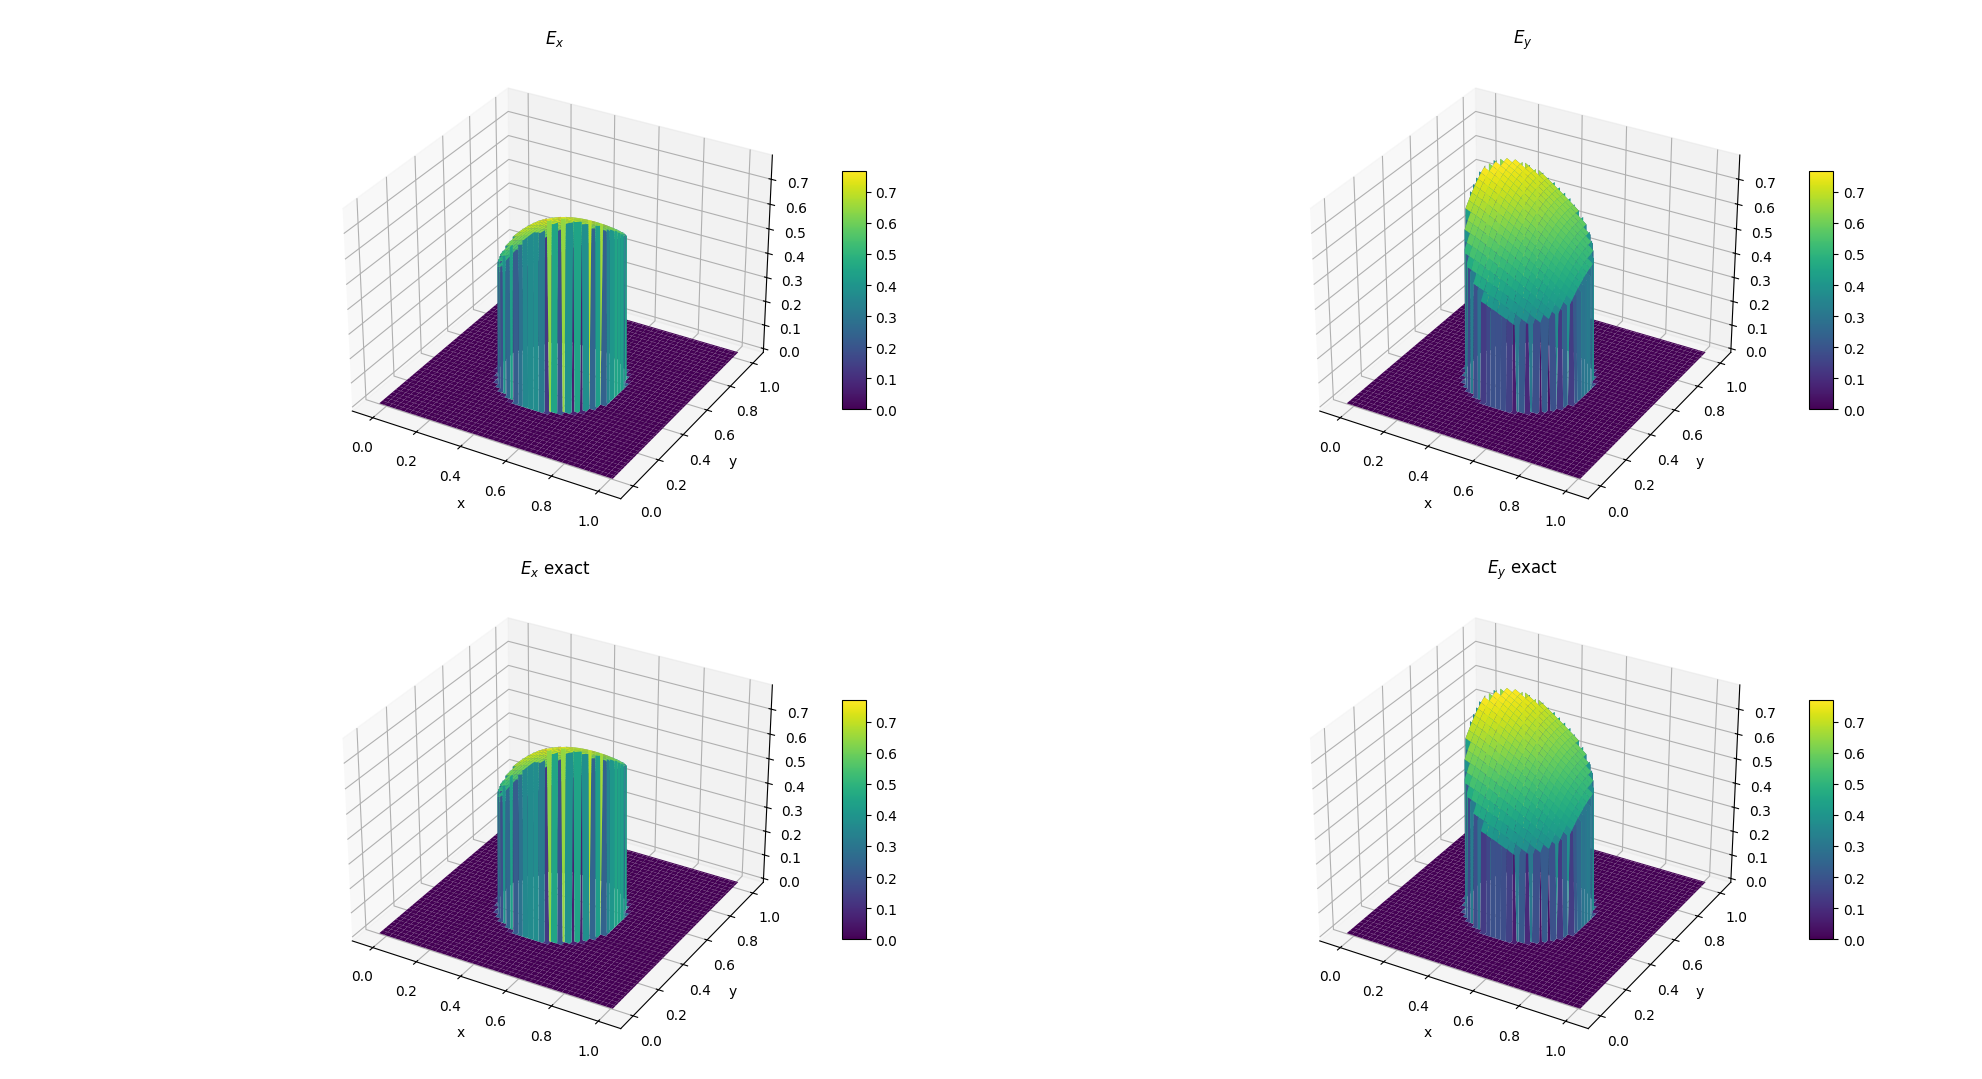
\includegraphics[width=\textwidth]{figures/poisson_gradient.png}
	\caption{Negative gradient of the numerical potential.}
	\label{fig:poisson_gradient}
\end{figure}

\begin{figure}[htbp!]
	\centering
	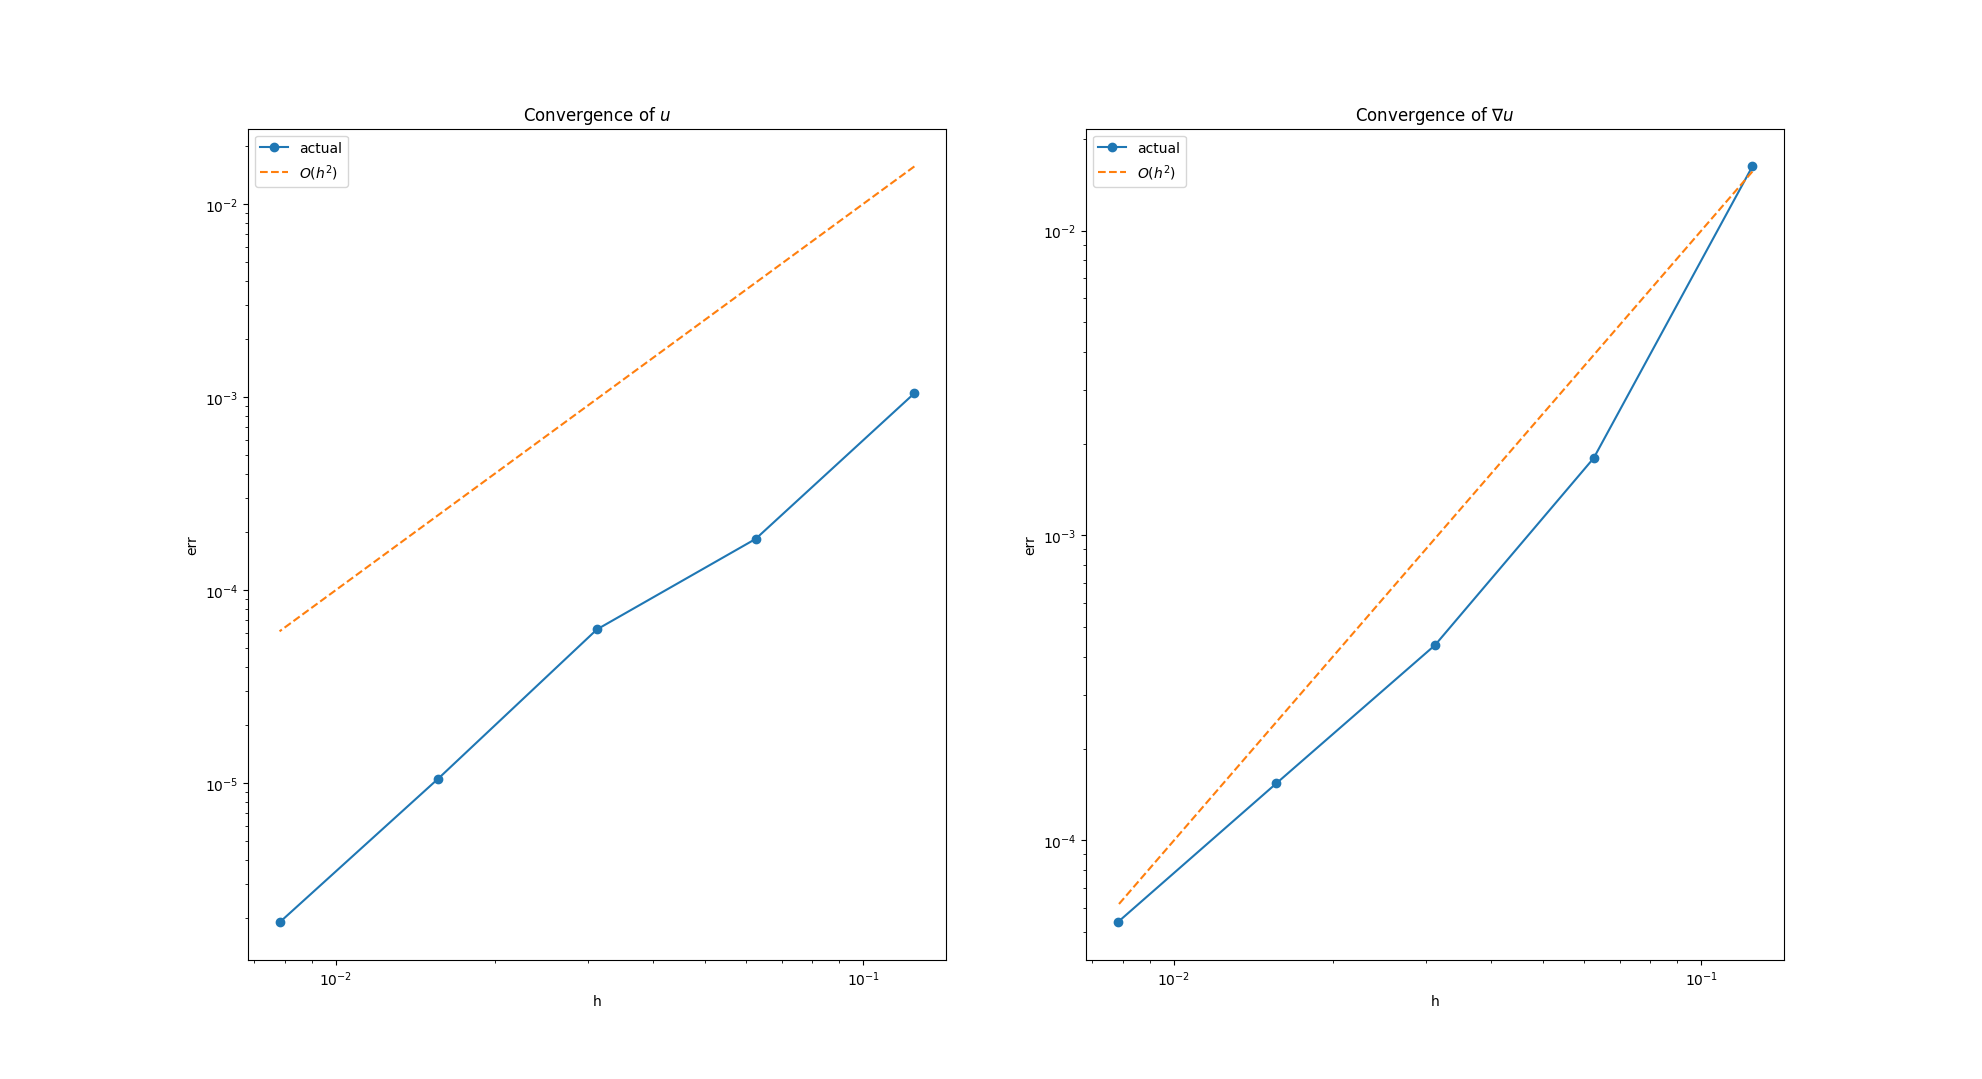
\includegraphics[width=0.95\textwidth]{figures/convergence_poisson.png}
	\caption{Convergence study for the Poisson equation with manufactured jump conditions.}
	\label{fig:poisson_convergence}
\end{figure}


\subsection{Test benchmarks}

After verifying the individual components (advection and Poisson), we now couple them and simulate two physically relevant problems.

\subsubsection{Plasma past a charged cylinder}

We consider a 2D2V Vlasov–Poisson system modelling a plasma flowing past a charged cylinder.  
The spatial domain is \((x,y)\in[0,L_x]\times[0,L_y]\), and the velocity domain is
\((v_x,v_y)\in[-5v_{th,i},\,15v_{th,i}]\times[-7v_{th,i},\,7v_{th,i}]\).  
The phase space is uniformly discretized with \((n_x,n_y,n_{v_x},n_{v_y}) = (160,50,120,50)\) interior cells and \(n_{\mathrm{gc}}=3\) ghost cells in each direction.  
The time step is \(\Delta t = 5\times10^{-4}\) and the final time is \(t_{\text{final}} = 0.15\).

Initially, no particles are present in the domain.  
Ions are injected through the left boundary via a shifted Maxwellian in \(v_x\) centred at \(v_x = 5v_{th,i}\).  
Zero inflow is imposed on the right boundary, and reflective conditions are used on the top and bottom boundaries.

Reference quantities are: \(x_0 = L_x\), \(m_0 = m_i\), \(n_0 = 1\;\text{m}^{-3}\), \(k_BT_0 = 0.15\;\text{eV}\).  
The charged cylinder is defined by \((x-0.375)^2 + y^2 = 0.125^2\).  
It is held at a potential \(\phi = -20\;\text{V}\); its permittivity is set to \(1000\) to mimic a conductor, while the surrounding vacuum has unity permittivity.  
The Poisson equation is solved with Dirichlet conditions on the inflow boundary (\(\phi=0\) at \(x=0\)) and homogeneous Neumann conditions elsewhere.

\begin{figure}[htbp!]
  \centering
  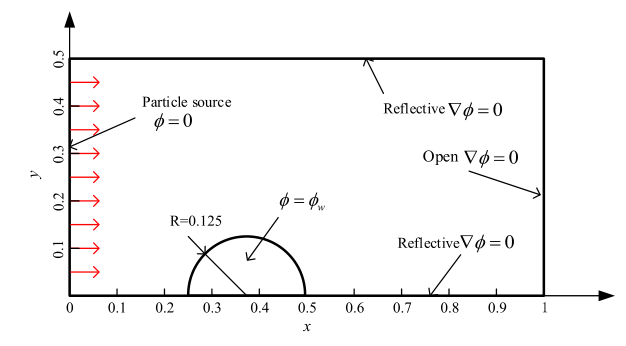
\includegraphics[width=0.7\textwidth]{figures/cylinder_setup.png}
  \caption{Schematic of the domain (normalised by \(L_x\)) and the boundary conditions.}
  \label{fig:cylinder_setup}
\end{figure}

\begin{figure}[htbp!]
	\centering
	\subfloat[Electric potential]{
		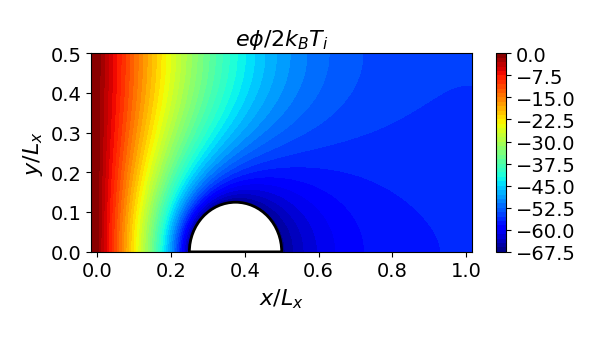
\includegraphics[width=0.5\textwidth]{figures/cylinder_potential.png}
	}
	\subfloat[Ion number density]{
		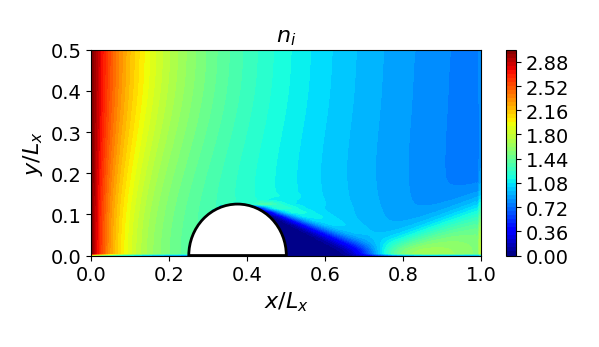
\includegraphics[width=0.5\textwidth]{figures/cylinder_number_density_ion.png}
	}
	\label{fig:cylinder}
\end{figure}

\subsubsection{Rough wall sheath problem}

Finally, we investigate the sheath formed near a wall with a rough surface.  
The spatial domain is \([0,20\lambda_D]^2\), where \(\lambda_D\) is the electron Debye length, discretised with \(n_x\times n_y = 100\times 50\).  
For electrons, the velocity space is \([-4v_{th,e},\,4v_{th,e}]\times[-5v_{th,e},\,5v_{th,e}]\) with \(v_{th,e}=\sqrt{k_BT_e/m_e}\); for ions, it is \([-4v_{th,i},\,4v_{th,i}]\times[-15v_{th,i},\,v_{th,i}]\) with \(v_{th,i}=\sqrt{k_BT_i/m_i}\).  
The time step is \(\Delta t = 0.015\) and the simulation runs for \(40\,000\) steps.  
Reference quantities are: \(L_0=\lambda_D\), \(m_0=m_e\), \(k_BT_0 = k_BT_e\), and \(T_i/T_e = 0.1\).

The wall consists of half‑circles, as shown in Fig.~\ref{fig:rough_wall_setup} (all dimensions are normalised by \(\lambda_D\)).  
On the wall, a Dirichlet condition \(\phi = -4\phi_0\) is imposed for the Poisson equation, and a zero‑inflow condition is used for the kinetic equations.

\begin{figure}[htbp!]
  \centering
  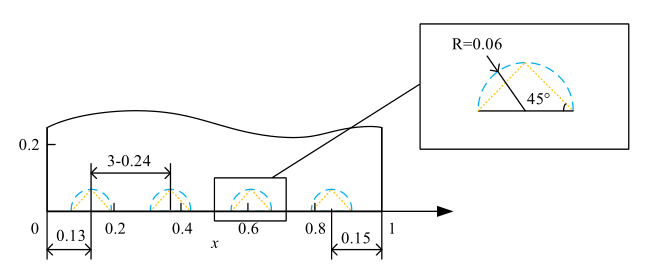
\includegraphics[width=0.7\textwidth]{figures/rough_wall_setup.png}
  \caption{Schematic of the rough wall domain (normalised by \(\lambda_D\)) and the boundary conditions.}
  \label{fig:rough_wall_setup}
\end{figure}

\begin{figure}[htbp!]
	\centering
	\subfloat[Electric potential]{
		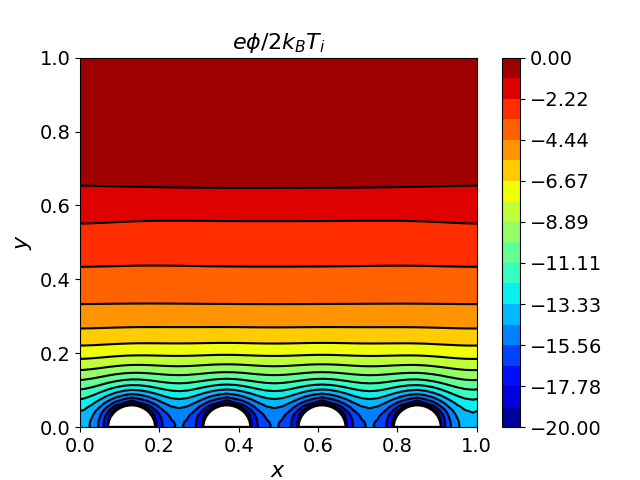
\includegraphics[width=0.5\textwidth]{figures/sheath_rough_wall_potential.png}
	}
	\subfloat[Electron number density]{
		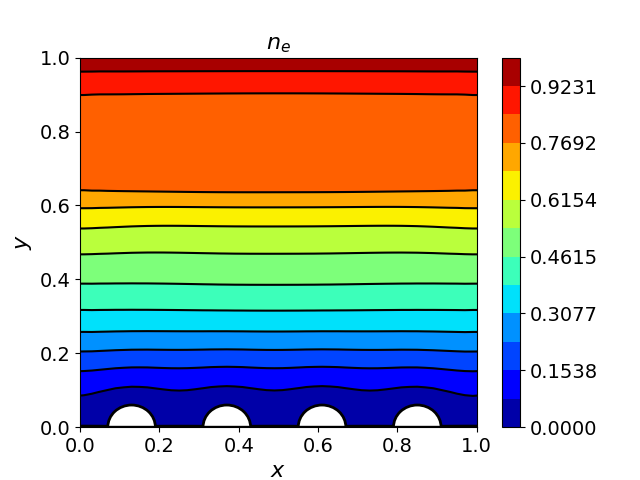
\includegraphics[width=0.5\textwidth]{figures/sheath_rough_wall_number_density_electron.png}
	}
	\label{fig:sheath_rough_wall}
\end{figure}
\section{Application Study}
A more realistic application case? (Compare with IFE-PIC)

\include{conclusion}



%% If you have bib database file and want bibtex to generate the
%% bibitems, please use
%%
%%  \bibliographystyle{elsarticle-num} 
%%  \bibliography{<your bibdatabase>}
\newpage
\bibliographystyle{elsarticle_num}
\bibliography{./ChenCui_Ref}

%% else use the following coding to input the bibitems directly in the
%% TeX file.

%% Refer following link for more details about bibliography and citations.
%% https://en.wikibooks.org/wiki/LaTeX/Bibliography_Management

% \begin{thebibliography}{00}

% %% For numbered reference style
% %% \bibitem{label}
% %% Text of bibliographic item

% \bibitem{lamport94}
%   Leslie Lamport,
%   \textit{\LaTeX: a document preparation system},
%   Addison Wesley, Massachusetts,
%   2nd edition,
%   1994.

% \end{thebibliography}
\end{document}

\endinput
%%
%% End of file `elsarticle-template-num.tex'.
